\tikzset{every picture/.style={line width=0.75pt}} %set default line width to 0.75pt        

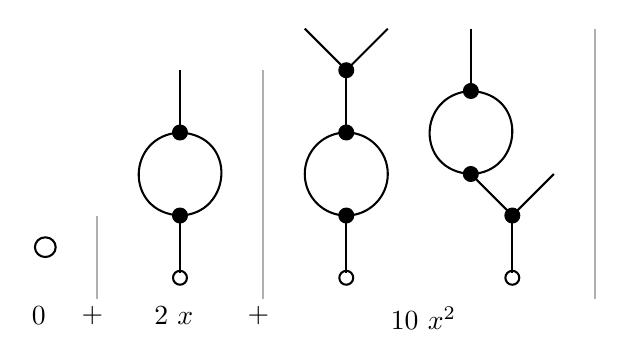
\begin{tikzpicture}[x=0.75pt,y=0.75pt,yscale=-1,xscale=1]
%uncomment if require: \path (0,183); %set diagram left start at 0, and has height of 183

%Shape: Circle [id:dp8438567026873804] 
\draw   (150,80) .. controls (150,68.95) and (158.95,60) .. (170,60) .. controls (181.05,60) and (190,68.95) .. (190,80) .. controls (190,91.05) and (181.05,100) .. (170,100) .. controls (158.95,100) and (150,91.05) .. (150,80) -- cycle ;
%Shape: Ellipse [id:dp46183104295319] 
\draw  [color={rgb, 255:red, 0; green, 0; blue, 0 }  ,draw opacity=1 ] (20,115.25) .. controls (20,112.63) and (22.24,110.5) .. (25,110.5) .. controls (27.76,110.5) and (30,112.63) .. (30,115.25) .. controls (30,117.87) and (27.76,120) .. (25,120) .. controls (22.24,120) and (20,117.87) .. (20,115.25) -- cycle ;
%Straight Lines [id:da9226208011234691] 
\draw [color={rgb, 255:red, 155; green, 155; blue, 155 }  ,draw opacity=0.8 ]   (130,30) -- (130,140) ;
%Straight Lines [id:da36667200859374194] 
\draw [color={rgb, 255:red, 0; green, 0; blue, 0 }  ,draw opacity=1 ]   (89.88,127.65) -- (89.88,100) ;
\draw [shift={(89.88,100)}, rotate = 270] [color={rgb, 255:red, 0; green, 0; blue, 0 }  ,draw opacity=1 ][fill={rgb, 255:red, 0; green, 0; blue, 0 }  ,fill opacity=1 ][line width=0.75]      (0, 0) circle [x radius= 3.35, y radius= 3.35]   ;
\draw [shift={(89.88,130)}, rotate = 270] [color={rgb, 255:red, 0; green, 0; blue, 0 }  ,draw opacity=1 ][line width=0.75]      (0, 0) circle [x radius= 3.35, y radius= 3.35]   ;
%Straight Lines [id:da02974694419719659] 
\draw    (89.88,30) -- (89.88,60) ;
\draw [shift={(89.88,60)}, rotate = 90] [color={rgb, 255:red, 0; green, 0; blue, 0 }  ][fill={rgb, 255:red, 0; green, 0; blue, 0 }  ][line width=0.75]      (0, 0) circle [x radius= 3.35, y radius= 3.35]   ;
%Straight Lines [id:da9697393736176018] 
\draw [color={rgb, 255:red, 0; green, 0; blue, 0 }  ,draw opacity=1 ]   (170,127.65) -- (170,100) ;
\draw [shift={(170,100)}, rotate = 270] [color={rgb, 255:red, 0; green, 0; blue, 0 }  ,draw opacity=1 ][fill={rgb, 255:red, 0; green, 0; blue, 0 }  ,fill opacity=1 ][line width=0.75]      (0, 0) circle [x radius= 3.35, y radius= 3.35]   ;
\draw [shift={(170,130)}, rotate = 270] [color={rgb, 255:red, 0; green, 0; blue, 0 }  ,draw opacity=1 ][line width=0.75]      (0, 0) circle [x radius= 3.35, y radius= 3.35]   ;
%Curve Lines [id:da45721750254801374] 
\draw    (89.88,60) .. controls (117.98,61.4) and (114.98,99.4) .. (89.88,100) ;
%Curve Lines [id:da02892604882157268] 
\draw    (89.88,100) .. controls (62.78,98.6) and (63.98,61.4) .. (89.88,60) ;
%Straight Lines [id:da47306464890332267] 
\draw    (170,30) -- (170,60) ;
\draw [shift={(170,60)}, rotate = 90] [color={rgb, 255:red, 0; green, 0; blue, 0 }  ][fill={rgb, 255:red, 0; green, 0; blue, 0 }  ][line width=0.75]      (0, 0) circle [x radius= 3.35, y radius= 3.35]   ;
\draw [shift={(170,30)}, rotate = 90] [color={rgb, 255:red, 0; green, 0; blue, 0 }  ][fill={rgb, 255:red, 0; green, 0; blue, 0 }  ][line width=0.75]      (0, 0) circle [x radius= 3.35, y radius= 3.35]   ;
%Straight Lines [id:da6003239891906188] 
\draw    (190,10) -- (170,30) ;
%Straight Lines [id:da0776145335231444] 
\draw    (150,10) -- (170,30) ;
%Straight Lines [id:da8790185641372728] 
\draw [color={rgb, 255:red, 0; green, 0; blue, 0 }  ,draw opacity=1 ]   (250,127.65) -- (250,100) ;
\draw [shift={(250,100)}, rotate = 270] [color={rgb, 255:red, 0; green, 0; blue, 0 }  ,draw opacity=1 ][fill={rgb, 255:red, 0; green, 0; blue, 0 }  ,fill opacity=1 ][line width=0.75]      (0, 0) circle [x radius= 3.35, y radius= 3.35]   ;
\draw [shift={(250,130)}, rotate = 270] [color={rgb, 255:red, 0; green, 0; blue, 0 }  ,draw opacity=1 ][line width=0.75]      (0, 0) circle [x radius= 3.35, y radius= 3.35]   ;
%Straight Lines [id:da32412310427320545] 
\draw    (230.03,10) -- (230.03,40) ;
\draw [shift={(230.03,40)}, rotate = 90] [color={rgb, 255:red, 0; green, 0; blue, 0 }  ][fill={rgb, 255:red, 0; green, 0; blue, 0 }  ][line width=0.75]      (0, 0) circle [x radius= 3.35, y radius= 3.35]   ;
%Curve Lines [id:da1836258760167958] 
\draw    (230.03,40) .. controls (258.13,41.4) and (255.13,79.4) .. (230.03,80) ;
%Curve Lines [id:da2215724554638565] 
\draw    (230.03,80) .. controls (202.93,78.6) and (204.13,41.4) .. (230.03,40) ;
%Straight Lines [id:da21245691821995005] 
\draw    (230,80) -- (250,100) ;
\draw [shift={(230,80)}, rotate = 45] [color={rgb, 255:red, 0; green, 0; blue, 0 }  ][fill={rgb, 255:red, 0; green, 0; blue, 0 }  ][line width=0.75]      (0, 0) circle [x radius= 3.35, y radius= 3.35]   ;
%Straight Lines [id:da6489375676218804] 
\draw    (250,100) -- (270,80) ;
%Straight Lines [id:da200020862588824] 
\draw [color={rgb, 255:red, 155; green, 155; blue, 155 }  ,draw opacity=0.8 ]   (50,100) -- (50,140) ;
%Straight Lines [id:da7133680859337238] 
\draw [color={rgb, 255:red, 155; green, 155; blue, 155 }  ,draw opacity=0.8 ]   (290,10) -- (290,140) ;

% Text Node
\draw (17,142.4) node [anchor=north west][inner sep=0.75pt]  [color={rgb, 255:red, 0; green, 0; blue, 0 }  ,opacity=1 ]  {$0$};
% Text Node
\draw (41,142.4) node [anchor=north west][inner sep=0.75pt]  [color={rgb, 255:red, 0; green, 0; blue, 0 }  ,opacity=1 ]  {$+$};
% Text Node
\draw (76,142.4) node [anchor=north west][inner sep=0.75pt]    {$2\ x$};
% Text Node
\draw (121,142.4) node [anchor=north west][inner sep=0.75pt]  [color={rgb, 255:red, 0; green, 0; blue, 0 }  ,opacity=1 ]  {$+$};
% Text Node
\draw (190,142.4) node [anchor=north west][inner sep=0.75pt]    {$10\ x^{2}$};


\end{tikzpicture}
